\chapter{Results and Comparisons}
\label{results}

In chapter~\ref{ch5}, the details of how the player tracking software works were discussed. In this chapter, the strategy for analysing the database discussed in chapter~\ref{database} as well as the additional tests are executed. Tests to determine the accuracy and reliability of the player tracking and log reading software  are also executed. The data from the results are then collected and analysed. The results are compared to the expected behaviour, and any irregular behaviour is explained. This is done in separate sections, one for the database analysis and one for the player tracking software analysis.

%Explain that the tests done, data collected and results gotten will be discussed for both database analysis and player tracking software in this chapter in different sections.


\section{Database Analysis}
To analyse the database, it is of interest to determine the following:

\begin{itemize}
	\item Which actions in the game generate queries.
	\item How many queries each action generates.
	\item The average amount of queries from a gaming session.
	\item How much queries increase with more players in the game world.
	\item Which queries are the most frequent.
	\item The inter arrival time of the most frequent queries.
	\item The queries that take the longest amount of time to execute.
	\item How the server responds when many players are logged in concurrently.
\end{itemize}

This data is then analysed to determine the data storage and retrieval behaviour of the server, as well as its behaviour during a typical gaming session of both one and many players.

\subsection{Database Tests}
At first the strategy described in chapter~\ref{datastrategy} was executed to determine which actions in the game generates which queries from the server. The queries generated by the server being started were also analysed. 

To test how queries are generated during typical gameplay, the game was played for three hours with one player logged in. The player did quests and upgraded skills and started professions as any normal player would do. This process was repeated a few times with different gameplay times and using different characters of different classes and races.

After the game was played with a single player, bots were added to simulate multiple players in the game world as was mentioned in chapter~\ref{further}. The bots were also selected as characters from different races and classes to make the queries generated as diverse as possible. The bots follow a predefined path, leaving the path to kill mobs of interest when the mobs come into range. They then looted the mobs and tried to get back onto the path they were following. 

This behaviour often caused bots to run into trees, rocks or houses causing them to get stuck. The bots therefore had to be constantly monitored to ensure that they did not get stuck and that they completed the quests that they were given. All the loot also had to be manually sold when the backpacks of the bots were full. 

The bots also played the game for approximately three hours, with the expected result of the generated queries being roughly four times as much as when one human player played the game. This experiment was repeated to get more data for analysing purposes.

%Explain the tests done, how bots were added etc. 

\subsection{Data Collection}

The logs that were generated and saved after each action was performed as discussed in chapter~\ref{datastrategy} were collected and analysed to determine the server behaviour. The logs contained all the queries that were generated, and in the case of logs that took longer than the slow query logs' minimum time, the time each query took was also saved. This same data was collected during the typical gaming session done by one player, and again when the experiment was repeated with bots added. 

MONyog was also used to gather server status data every five minutes during the gameplay of these tests. This generated queries of its own, but these were ignored during analysis. The status data can not be saved in the same way that the logs can, so the data had to be used to create graphs immediately after each test was done, before new and irrelevant status data was captured by MONyog.



%The data required is information about which queries were made by the clients throughout the gaming session, as well as what time the queries were made and how long the queries took. The data was collected separately for the different tests done by activating the general and the slow query log. The logs were then saved and cleared after each test in order to start the next test with a clean log. MONyog was also used to gather server status data every five minutes during the gameplay. This generates queries of its own, but these were ignored when analysing the logs.
%
%The status data can not be saved in the same way that the logs can, so it had to be used to create graphs immediately after each test before new and irrelevant status data was captured by MONyog.


%Explain how data was collected and show results. 

\subsection{Results}
The results of the tests to determine which actions in WoW caused the server to generate queries was first analysed to better understand how the server responds to different actions, before the typical gameplay results were analysed.

\subsubsection{Wow Queries}

What was surprising after analysing the logs after each action was performed, was that most of the actions performed by the character did not generate immediate queries. The expected queries did however happen  a few seconds or even minutes after the action was performed. This suggests that the server saves all actions that will generate queries in variables at first. A queue of queries is then created that is executed either when the queue gets too full or after a certain interval. There are however certain actions that always generated immediate queries. This could mean that those queries are either big enough for the queue of queries to be considered full enough to be executed, or they are simply of higher priority and thus handled immediately. When these queries are executed however, the queries that were generated by performing other actions were still not executed, which rules out the theory of the server having a queue of queries that gets executed whenever it gets full.

Extensive testing was done to test this server behaviour, and after generating as much queries as possible with five clients logged in simultaneously, the queries still only happened after a counter of sorts triggered the queries to be made. This suggests that the server has a timer that generates an interrupt after a set amount of time has passed. This interrupt then causes the server to make all the queries from actions that have heaped up to the database. This is the equivalent of saving all the changes that have happened in the meantime.

It is sensible for the server to behave in this way, because the server has a lot of other things that it is responsible for, such as generating all the actions of the mobs and sending location information to all the clients and so forth. If every action that caused a change in game state generated an immediate query then the server would constantly be busy sending information to the database, causing lag in its normal and more important function of communicating with the client. This behaviour would become worse when more clients connect to the server, and the game would soon become unplayable. 

The following pattern was discovered by analysing hundreds of queries made to the database to ensure its legitimacy: there are two counters that generate queries constantly looping on the server side. The one counter generates a query to check if any of the players has sent mail to any of the other players every three minutes. This is the shorter of the two counters, which is understandable because other players could be waiting for the mail to be sent, which makes it a higher priority query.

The other counter generates a ``START TRANSACTION'' query every five minutes. This query starts a sequence of queries that save all the changes to all the characters that have happened in the past five minutes. This includes all new skills and spells learned, gold collected, quests accepted and completed and so forth. 

Table~\ref{queries} lists all the actions that were found to generate queries immediately, as well as the amount of queries that they generate. The queries generated by starting the ArcEmu server are also listed. Starting ArcEmu generates the largest amount of queries by far, but this should only happen once per week at a maximum, when servers are restarted for maintenance purposes.


\begin{table}[htbp]
  \centering
  \caption{List of actions in WoW that generate immediate queries}
    \begin{tabular}{lrlr}
    \addlinespace
    \toprule
    \textbf{Action in game} & \textbf{} & \textbf{Queries} & \textbf{Total time to execute} \\
    \midrule
    Starting ArcEmu &       & 1845 queries & 27.199 sec \\
    \midrule
    Logging in &       & 3 queries & 1.047 sec \\
    \midrule
    Creating a character &       & 18 queries & 0.765 sec \\
    \midrule
    Entering World &       & 23 queries & 0.597 sec \\
    \midrule
    Selling Items &       & 1  query & 0.056 sec \\
          &       & per item &  \\
    \midrule
    Dying &       & 2 queries & 0.059 sec \\
    \midrule
    Resurrecting &       & 1  query & 0.049 sec \\
    \midrule
    Logging Out &       & 76 queries & 0.078 sec \\
    \bottomrule
    \end{tabular}%
  \label{queries}%
\end{table}%


All of these actions in WoW are of high priority, which is why the server deems them important enough to break its usual cycle of only saving changes to the database every few minutes. Most of these actions only happen once per gaming session, or at the least they happen far less than other actions, so they should not have an adverse effect on the performance of the server.

The actions in the game that happen most frequently, like gaining skill points, levelling up and starting and completing quests are all processed at the same time, and only add one query per action to the list. Attributes like which spells a character knows and which items are in their backpacks are all both deleted and inserted into the database every five minutes with the ``START TRANSACTION'' query that happens. This will happen even if the character does nothing in that time. Analysing several logs revealed that the ``START TRANSACTION'' query generates approximately 66 queries for every player every 5 minutes when the player does nothing and is still low level. This sounds like a lot, but out of the 66 queries only 10 appeared in the slow query log, which means that 56 of them took faster than 0.000001 seconds to execute. 
The ``START TRANSACTION'' queries took a total of  0.095 seconds to execute.

\subsubsection{Typical Gameplay Analysis}

After analysing how the server handles queries, it is still of interest to determine if this behaviour persists when a player plays the game for long, and if the amount of queries multiplies when more players are added. The data of the one person playing and the bots playing was thoroughly investigated and it was found that the amount of queries and their size was mostly consistent with what was expected.

The game with one player in it will be referred to as game 1 from now on, and the game with four bots in it will be referred to as game 2.

The behaviour of the server suggested that queries should mostly happen every five minutes during gameplay, with the amount of queries from game 2 expected to be roughly four times as much as that of game 1.

From the time in the logs it was determined that game 1 lasted 205 minutes while game 2 lasted 218 minutes. There were 40 ``START TRANSACTION'' and 69 ``SELECT * FROM mailbox\_insert\_queue'' queries in game 1, and 157 ``START TRANSACTION'' and 73 ``SELECT * FROM mailbox\_insert\_queue'' queries in game 2. Table~\ref{botsres} shows the inter-arrival time of these queries for each of the queries in the two games.



\begin{table}[htbp]
  \centering
  \caption{Inter-arrival times for start transaction and mailbox insert queue queries}
    \begin{tabular}{lrr}
    \addlinespace
    \toprule
    \textbf{Queries} & \textbf{Game1} & \textbf{Game 2} \\
    \midrule

    START TRANSACTION & 5.125 min & 1.388 min \\
    \midrule
    SELECT * FROM mailbox\textbackslash \_insert\textbackslash \_queue & 2.971 min & 2.986 min \\
    \bottomrule
    \end{tabular}%
  \label{botsres}%
\end{table}%

As can be seen from table~\ref{botsres}, the start transaction query happened every 5 minutes as expected for game 1, and the other query also happened every 3 minutes as expected. In game 2, the one query behaved as expected, but the start transaction queries happened much more frequent than expected. This means that the server starts a separate timer for each character that logs into the game and saves their separate values to the database every five minutes. The reason that the inter arrival times are not exactly four times less than in game 1, is because it took a while to set up all the bots correctly, so the game was started with only one bot at first and the rest being added one by one every few minutes.

The logs of both games were processed next, to determine the top five most frequent queries and their inter-arrival times, as well as the queries that took the longest time to execute. Table~\ref{amount} shows the five most frequent queries and the amount of times they were executed during the games. The amount of times they were executed in game 2 is roughly three times as much as in game 1. The reason that it is not closer to four as expected is that the bots can not play the game as efficiently as a real player and therefore the amount of skills and so forth that the human player gained is much more than the bots could manage.

\begin{table}[htbp]
  \centering
  \caption{The amount of times the five most frequent queries were executed}
    \begin{tabular}{lrr}
    \addlinespace
    \toprule
    \textbf{Queries} & \textbf{Game 1} & \textbf{Game 2} \\
    \midrule
    INSERT INTO playerspells & 2313  & 7922 \\
    \midrule
    INSERT INTO playerskills & 548   & 1839 \\
    \midrule
    DELETE FROM playeritems & 421   & 1296 \\
    \midrule
    INSERT INTO playeritems & 237   & 908 \\
    \midrule
    DELETE FROM questlog & 192   & 517 \\
    \bottomrule
    \end{tabular}%
  \label{amount}%
\end{table}%

The inter-arrival times of the most frequent queries are shown in table~\ref{interamount}.

\begin{table}[htbp]
  \centering
  \caption{The inter-arrival times of the five most frequent queries}
    \begin{tabular}{lrr}
    \addlinespace
    \toprule
    \textbf{Queries} & \textbf{Game 1} & \textbf{Game 2} \\
    \midrule
    INSERT INTO playerspells & 0.089 min  & 0.027 min \\
    \midrule
    INSERT INTO playerskills & 0.374 min   & 0.118 min \\
    \midrule
    DELETE FROM playeritems & 0.487 min   & 0.168 min \\
    \midrule
    INSERT INTO playeritems & 0.865 min   & 0.240 min \\
    \midrule
    DELETE FROM questlog & 1.067 min   & 0.412 min \\
    \bottomrule
    \end{tabular}%
  \label{interamount}%
\end{table}%

Comparing the general and slow query logs, there are 4590 queries in total in the general log of which 514 appear in the slow query log for game 1. The other game has  15286 queries in the general log of which 2017 appear in the slow query log. This means that in both cases, less than 15\% of the queries generated takes longer than 0.000001 seconds to execute.

The query ``INSERT INTO character\_achievement\_progress'' took 0.35 seconds to execute, which was the longest query present in game 1. These queries happen often, yet only one took this long, so the reason is most probably that the computer was busy processing some other application which made the query take longer. For game 2 the longest query was a SELECT query, executed when a player logged into the world, which took 0.641 seconds to execute. This happened while the computer was busy running 4 instances of the game, which would keep the processor occupied and explains this long query time.

MONyog sent queries to the database every five minutes to check its status and saved the results temporarily. These results were used to draw figures for both game 1 and game 2, which are shown and compared next. To make game 1 reflect the behaviour expected from a normal player and to show what happens when no players are logged into the game, the character was signed off for a 15 minute break in the middle of the total game time. This can clearly be seen in figures~\ref{diffqueries}, \ref{rowaccess} and \ref{totalqueries}.

\begin{figure}[htbp]
\centering
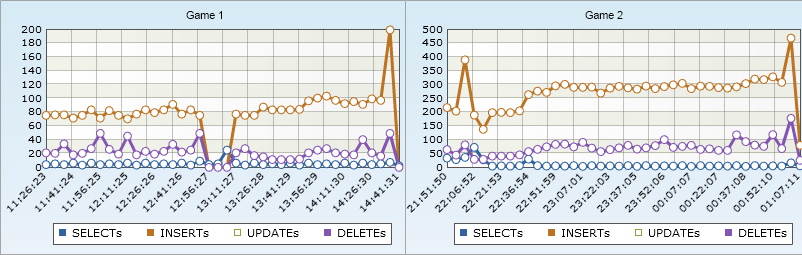
\includegraphics[scale = 0.75]{statecomp.png}	
\caption{Different queries over time for both games}
\label{diffqueries}
\end{figure}

Figure~\ref{diffqueries} shows the amount of different queries made during the two games. This result reflects the earlier result of the most frequent queries, with game 2 having roughly 3 times as much of each different query throughout the game.

\begin{figure}[htbp]
\centering
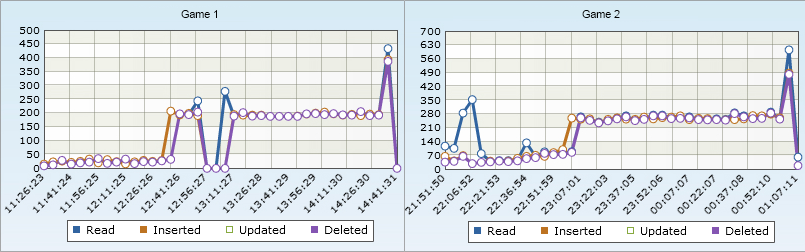
\includegraphics[scale = 0.75]{rowcomp.png}	
\caption{Different row access amounts over time for both games}
\label{rowaccess}
\end{figure}

Figure~\ref{rowaccess} shows the amount of rows that were accessed throughout the two games. The reason for the sudden jump in both games is that the character achievement progress query suddenly becomes more when the player levels up and learns more skills and spells. This query goes from accessing 0 rows, to 9 rows and then suddenly to 182 rows after levelling up and learning spells. The values in game 2 is not much more than in game 1 because the bots could not level up their characters enough to be able to do this. The rows being accessed by each of their queries stayed less than 20, and the only reason for the spikes that are seen in the graph is that the same character that was used in the first game was entered as a bot in the second game. This fact was taken into account when analysing the queries.

This is an interesting result to note however, especially since the size of the queries are of interest. The only way to judge the size of the query is by looking at the amount of rows accessed, of which all the other queries are dwarfed by the character\_achievement\_progress and the playerspells queries. The reason that they get so big is that a lot of new skills and spells can be learned by characters as they level up. These new skills and spells are probably each in a different row in their respective tables, causing the rows that need to be accessed to increase severely as the player progresses through the game.


\begin{figure}[htbp]
\centering
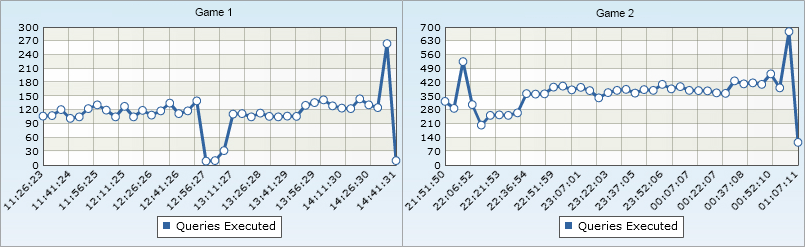
\includegraphics[scale = 0.75]{queriescomp.png}	
\caption{Total amount of queries executed for both games}
\label{totalqueries}
\end{figure}

Figure~\ref{totalqueries} shows the total amount of queries executed throughout the games. The value of game 2 is slightly more than 3 times as much as that of game 1 as expected. The reason it is not 4 times as much is once again that the bots can not play the game as efficiently as a human can, which resulted in less quests being completed and less skills and spells learned, which in turn resulted in less queries being executed.




%Discuss results, compare to what was expected and explain differences.

\section{Player Tracking Software Analysis}

To analyse and test the player tracking software, it is of interest to determine the following:

\begin{itemize}
	\item Whether the software reads the memory locations as expected.
	\item Whether the coordinates of the local player is the same as it is from another character using the software.
	\item Whether the traces created reflects true player movement data.
	\item Whether the log reading program recreates the traces correctly from logs.
	\item Whether the the tracking information in general is correct.
\end{itemize}

To determine this, tests need to be done and data collected.

\subsection{Player Tracking Tests}

The first test needs to determine whether the tracking software reads the memory of the WoW client properly. It was explained in chapter~\ref{ch5} how the data structure of WoW looks and how the software extracts the proper data from the memory. Figure~\ref{objalone} shows that a copy of the GUID of the local player is accessible directly from the object manager, which is then used to gain access to the object representing the local player, as shown in figure~\ref{getbase}. This same method is used to get access to the object representing the currently selected target. To test whether the tracking software reads the data structure correctly, and more importantly whether the data structure works as expected, a user must enter the game while using the player tracking software. The user must then select himself, making the local player the currently selected target. The software should then show the same name, GUID and coordinates for the local player and the target.

% Another copy of the GUID of the local player should be in the object that represents the local player in the object manager. These two values must be read from memory and compared to each other to test if the software reads the memory of the WoW client correctly. As an added test, the current player must be selected as the current target. This should create yet another copy of the GUID of the local player to be read and compared to the rest.

What needs to be tested next is whether the data shown graphically by the software reflects what the player sees in the game. The player must log into the game while using the software and compare the NPCs and other players it sees in the game to what NPCs and players the software says is around it. The names of the NPCs shown in game must also be compared to the names shown by the tracking software, as well as the data of the current target.

This test should prove that the data read on one computer is correct and consistent, but another test is needed to ensure that different players receive the same data. To test this, two different clients must log into WoW with different characters while using the tracking software. The two characters must then select each other as targets, and compare the information displayed about themselves and their targets by the software with each other. The target information from the one player should match the local player information of the other player exactly.

While having two payers logged in, the player tracing feature should be tested by enabling the feature with one player, and using the other player to move in a shape. The shape should then be reflected perfectly on the player tracking software. The other player should then be selected to make him a target, and another shape should then be drawn by moving, which should then be displayed in red.

Lastly, the usability and performance of the software must be tested when large amounts of players are tracked simultaneously. This test must be done in densely populated areas such as capital cities to get good test data. Traces should then be formed and compared to maps of the area to see if the movement data makes sense. 

%Briefly mention tests done to ensure program works again.

\subsection{Data Collection}
Data needs to be collected to prove that the software works accurately and as expected. To do this, the various tests mentioned need to be performed with screenshots of the game window and of the software being taken to prove that they were done and that they were successful. 

Data also needs to be collected about tracking large amounts of players. For this purpose the logs that the program creates must be collected and compared with what happened in the game to see if the data reflects what happened. The maps of the area must also be compared with traces of player movement data to see if the movement traces make sense and can be explained on the game map. This data must also be compared to what is happening in the game. 

Video footage of what happens in the game must be taken to compare to the results in the logs and the traces shown. This will allow any inconstancies to be explained by studying the video of the game. Screenshots and videos of the traces made in real time also need to be collected for comparison to traces recreated from logs, to see if the two are the same. After all this data has been collected, it needs to be analysed thoroughly to prove that the software works as expected.
%Mention how data was collected and show results

\subsection{Results}
\label{trackingresults}
It is of vital importance that the data structures of WoW are both understood correctly, and that the program reads them correctly. This was tested by selecting the local player, making it the current target. If everything works as it should, the software should have access to the local GUID, the target GUID and all the objects as shown in figure~\ref{test1}. The right objects must then be found by comparing the GUID that is already accessed with each object as is shown in figure~\ref{getbase}.


\begin{figure}[htbp]
\centering
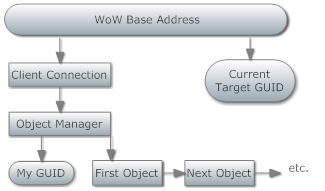
\includegraphics[scale = 0.75]{test1.png}	
\caption{The data structure that the player tracking software must use}
\label{test1}
\end{figure}

In WoW, the name, health, mana, level and a small picture of both the local player and the current target are shown in the top left corner of the UI as shown in figure~\ref{self2}. The local player is represented on the left, and the target on the right. Figure~\ref{self2} clearly shows that the local player is currently selected as the target in the game.

\begin{figure}[htbp]
\centering
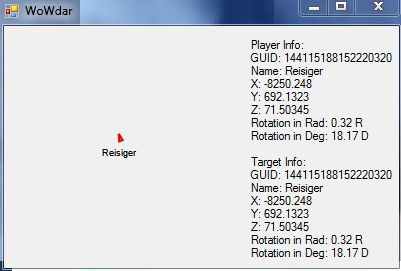
\includegraphics[scale = 0.75]{self1.png}	
\caption{Player tracking software with local player as target}
\label{self1}
\end{figure}

Figure~\ref{self1} shows the player tracking software with the local player selected as target. All irrelevant data has been edited out of the GUI in order to clearly show that the player and target information displayed in the tracking software are exactly the same. This includes the name, GUID, coordinates and rotation values.

\begin{figure}[htbp]
\centering

\includegraphics[scale = 0.75]{self2.png}	
\caption{The local player selected as the current target}
\label{self2}
\end{figure}

This is considered proof that the data structures of WoW works as explained. Next it needs to be confirmed that what the tracking software displays is reflected in the game world. To do this, an NPC is approached and targeted. The name, rotation and position of the NPC is compared to the same values displayed by the tracking software. Figure~\ref{target1} shows the local player standing in front of an NPC called Marshal McBride. A Stormwind Royal Gaurd can also be seen to the left. Both NPCs are looking in the opposite direction of the local target.

\begin{figure}[htbp]
\centering
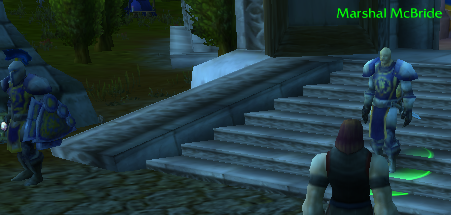
\includegraphics[scale = 0.75]{target11.png}	
\caption{An NPC is approached and targeted in the game}
\label{target1}
\end{figure}

Figure~\ref{target2} shows the tracking software view of the same moment in the game. The green arrow represents the local player, while the red one represents the current target, and all the plum ones are NPCs. Figure~\ref{target2} shows that the orientation of the NPCs, as well as their names, are an exact representation of what is shown in the game world.

\begin{figure}[htbp]
\centering
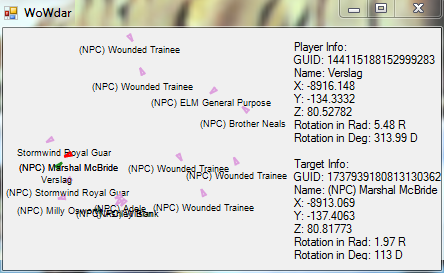
\includegraphics[scale = 0.8]{target12.png}	
\caption{Player tracking software showing an NPC being approached and targeted}
\label{target2}
\end{figure}

Now that it has been proved that the data received by one player using the software is consistent with what is represented in the game, it needs to be proven that different players using the software will also receive the exact same data. This is done by logging into the game with two different players, meeting each other in the game with the tracking software open for each player respectively, and selecting each other as targets. The target information of the one player should then be exactly the same as the local player information of the other player. Figure~\ref{ektarget2} shows the two players, Reisiger and Verslag,  meeting up in the game. 

\begin{figure}[htbp]
\centering

\includegraphics[scale = 0.75]{ektarget2.png}	
\caption{Two players meeting up in the game world}
\label{ektarget2}
\end{figure}

The information displayed by the tracking software of Reisiger is shown in figure~\ref{ektarget1}. The target information should be exactly the same as the local player information displayed by the tracking software of Verslag.

\begin{figure}[htbp]
\centering
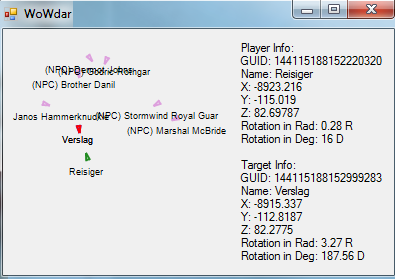
\includegraphics[scale = 0.8]{ektarget1.png}	
\caption{The tracking software display of Reisiger}
\label{ektarget1}
\end{figure}

The information displayed by the tracking software of Verslag is shown in figure~\ref{targetek1}. As can be seen from figures~\ref{targetek1} and \ref{ektarget1}, the information is displayed exactly as expected, with the name, GUID, coordinates and rotation being an exact replica of each other. This proves that the tracking software extracts and displays consistent and accurate values for all its users.

\begin{figure}[htbp]
\centering
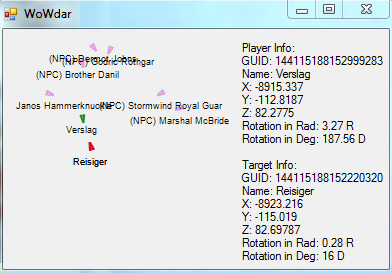
\includegraphics[scale = 0.8]{targetek1.png}	
\caption{The tracking software display of Verslag}
\label{targetek1}
\end{figure}

With the two players still logged in together, the show traces feature was tested by enabling the feature on one player's software, while the other player moved around in a specific way to form a shape. The shape should then be reflected on the player tracking software in blue. The player was then selected as the target before drawing yet another shape by moving. The trace made by a target should then be displayed in red. Figure~\ref{vierkant} shows the resulting display of the tracking software after the test was performed, with the square being made before the player was selected and the circle afterwards. The trace shows half a circle being formed unsuccessfully before the circle was then completed. This is an accurate representation of the player running into a tree before starting a circle without obstacles in the way. The circle is also not completely round, and the reason for this is that the player was riding a horse that galloped in that form when trying to run in a circle.


\begin{figure}[htbp]
\centering
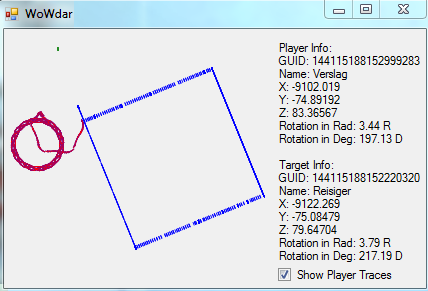
\includegraphics[scale = 0.75]{vierkant1.png}	
\caption{The traces made by moving around a player in certain shapes}
\label{vierkant}
\end{figure}

The accuracy of the log reading program also needs to be tested. To do this, the two players that are logged in simultaneously are used again. The one player moves in the shape of a triangle while the other player enabled both the tracking and the show traces features. The trace shown by the player tracking software must then be compared by the trace created by the log reading program when it reads the log created after the player moved in a triangle. Figure~\ref{tracetest1} shows the trace made by the tracking software, while figure~\ref{tracetest2} shows the trace made by the log reading software. The two forms are exactly the same, which proves that the log reading software can accurately read the logs and display the information they contain. It also proves that the player tracking software creates the logs properly, with no data being lost.

\begin{figure}[htbp]
\centering
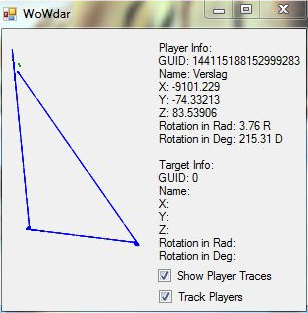
\includegraphics[scale = 0.75]{tracetest.png}	
\caption{The trace made by the tracking software}
\label{tracetest1}
\end{figure}

\begin{figure}[htbp]
\centering
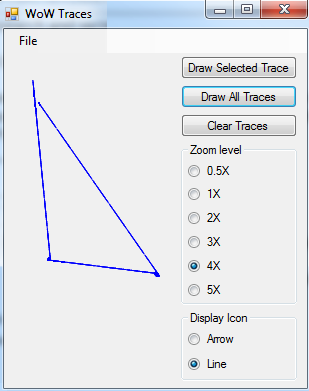
\includegraphics[scale = 0.75]{tracetest2.png}	
\caption{The trace made by the log reading software}
\label{tracetest2}
\end{figure}

Finally the performance and accuracy of the tracking software needs to be tested when there are many players to track. This is done by going into a city and enabling both the player tracking and the show traces features. The traces are then overlaid on a map to see if the movement data represented makes sense. Figure~\ref{stormtrace} shows the player traces captured in the city of Stormwind overlaid on the map of Stormwind. The auction house, bank and some flying mounts have been pointed out in figure~\ref{stormtrace}. A lot of traffic can be seen between the auction house and the bank. This is because players either buy an item at the auction house and then store it in the bank, or they get an item from the bank to sell at the auction house. The traces clearly follow the streets of the city, which can clearly be seen at the bridges, except in the case of flying mounts, which can fly over all the buildings.

\begin{figure}[htbp]
\centering
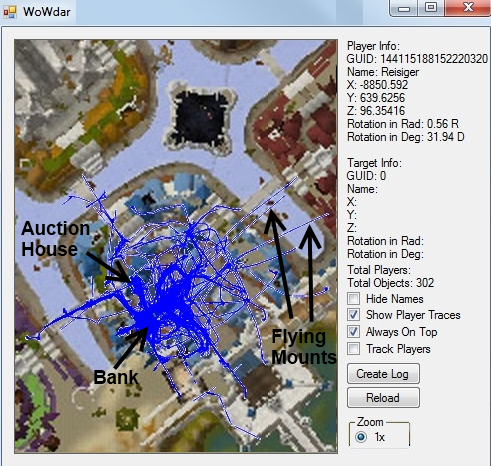
\includegraphics[scale = 0.75]{stormoverlay.png}	
\caption{Player traces overlaid on the map of Stormwind}
\label{stormtrace}
\end{figure}

Another test was done in the city called Undercity. The player traces overlaid on the map of Undercity is shown in figure~\ref{undertrace}. Undercity is an underground city as the name suggests, and therefore the movement of players with flying mounts are very limited. The green that can be seen is water, which players can enter if they want to, but it slows down movement. The rest of the map is mostly walkways, roads and walls. The trace shows that the players use the roads and walkways provided almost exclusively.

\begin{figure}[htbp]
\centering
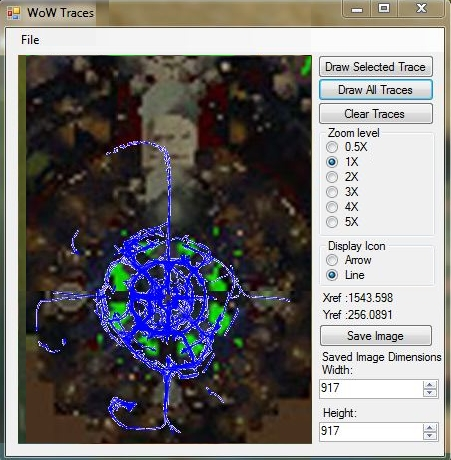
\includegraphics[scale = 0.75]{underlaycity.png}	
\caption{Player traces overlaid on the map of Undercity}
\label{undertrace}
\end{figure}

The traces shown in figures~\ref{undertrace} and \ref{stormtrace} contains no inexplicable movement data, which is considered proof that the player tracking software works efficiently and accurately in densely populated areas where a lot of players need to be tracked.


%Discuss results and compare with expected results and explain differences.

